\documentclass[a4paper]{article}
\def\DOCTITLE{CSC3424 Bio Algorithms}
% Set document attributes
\title{\DOCTITLE}

\usepackage{fullpage}
\usepackage{scrextend}
\usepackage{titlesec}
\usepackage{fancyhdr}
\usepackage{amsmath}
\usepackage{amssymb}
\usepackage[section]{placeins}
\usepackage{booktabs}
\usepackage{hyperref}
\usepackage{tikz}
\usepackage{graphicx}
\usepackage{minted}
\usepackage{subcaption}

% Setup headers and footers
\pagestyle{fancy}
\lhead{}
\chead{\DOCTITLE}
\rhead{}
\rfoot{}
\cfoot{\thepage}
\lfoot{}

% New page for each section
\newcommand{\sectionbreak}{\clearpage}

% Set header and footer sizes
\renewcommand{\headrulewidth}{0.4pt}
\renewcommand{\footrulewidth}{0.4pt}
\setlength{\headheight}{15.2pt}
\setlength{\headsep}{15.2pt}

\setlength{\parskip}{5pt plus 1pt minus 1pt}
\setlength{\parindent}{0pt}

% Newline after paragraph
\newcommand{\Para}[1]{\paragraph{#1}\mbox{}}

% Stuff used in cryptography notes
\newcommand{\Forall}{\;\forall\;}
\newcommand{\Mod}{\: mod \:}

% Stuff used in distributed systems notes
\newcommand{\happenbefore}{\rightarrow}
\newcommand{\orderbefore}{\Rightarrow}
\newcommand{\clockcond}{\leadsto}
\newcommand{\RArrow}{$\rightarrow$}

\def\checkmark{\tikz\fill[scale=0.4](0,.35) -- (.25,0) -- (1,.7) -- (.25,.15) -- cycle;}


\begin{document}

\tableofcontents

\section{Cell and Molecular biology}

\subsection{The Cell}

\begin{itemize}
  \item Minimal unit of life
  \item Cell is a system of many components enclosed in a series of membranes
  \item Small organisms such as fungi and bacteria are unicellular
  \item Plants and animals are generally multicellular
\end{itemize}

\subsubsection{Prokaryotes}

\begin{itemize}
  \item All prokaryotes are single cell
  \item Smaller than eukaryotic cells \\
        ($< 1 \mu \mathrm{m}$ in diameter)
  \item Simple structure \\
        No inner cellular membranes
  \item Very adaptable to environment \\
        Found in almost every habitat
  \item Approximately $5x10^{30}$ prokaryotic cells in the world
  \item Essential for healthy life
\end{itemize}

\Para{Prokaryotic cell}

\begin{itemize}
  \item Less complex than eukaryotic cells
  \item Contain no organelles
  \item Believed to represent the earliest life on earth and that eukaryotic
        cells evolved from prokaryotic cells
\end{itemize}

\begin{figure}[h!]
  \centering
  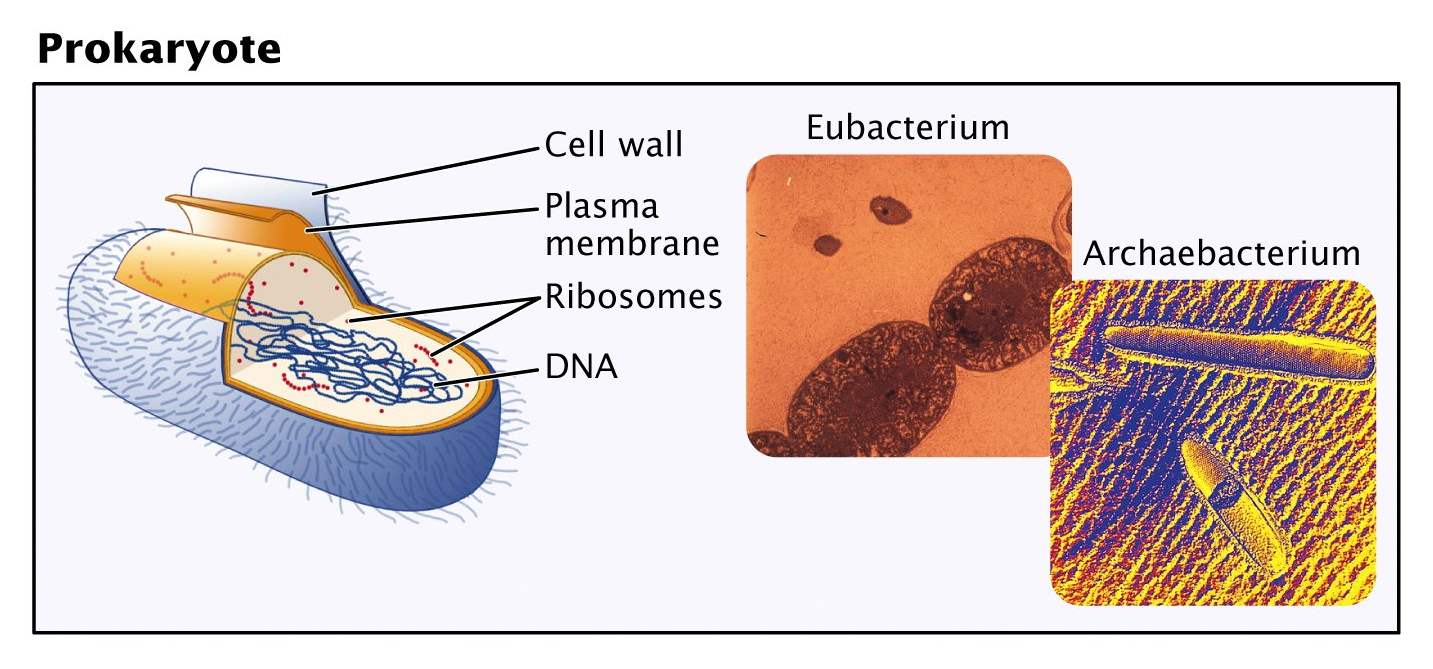
\includegraphics[width=0.7\textwidth]{graphics/prokaryotic_cell.eps}
  \caption{Prokaryotic cell structure}
  \label{fig:prokaryotic_cell}
\end{figure}
\FloatBarrier

\Para{Types of prokaryotes}

Types descend from common ancestor.

\begin{description}
  \item[Eubacteria] \hfill \\
    Common bacteria that affects life daily
  \item[Archaea] \hfill \\
    Tend to exist in extreme habitats (high pressure, temperature, pH)
\end{description}

\subsubsection{Eukaryotes}

\begin{itemize}
  \item More structurally and biochemically complex than prokaryotes
  \item Evolutionarily more recent
  \item Believed to have evolved through endosymbiosis
\end{itemize}

\begin{figure}[h!]
  \centering
  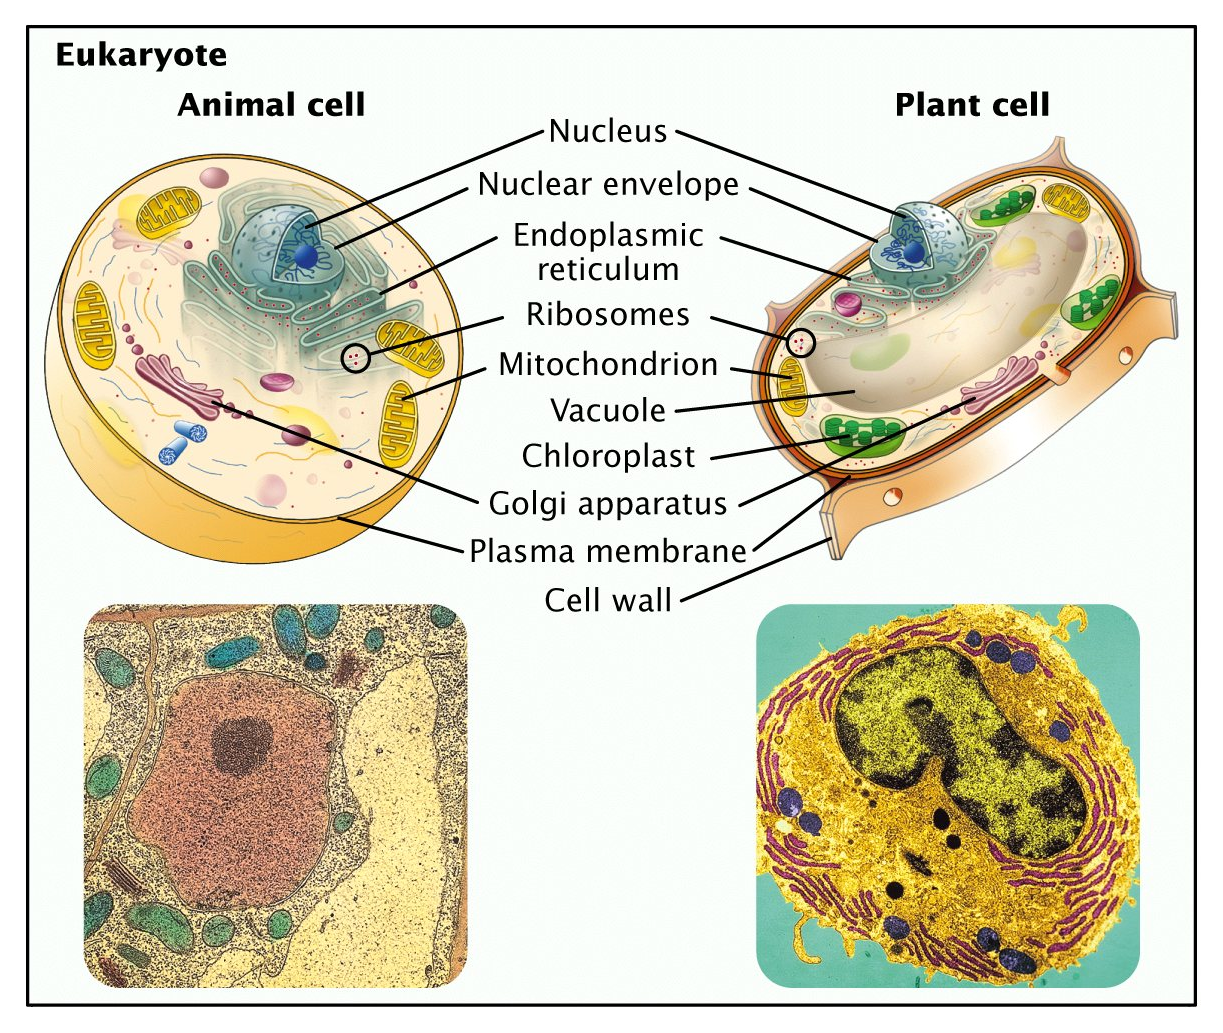
\includegraphics[width=0.7\textwidth]{graphics/eukaryotic_cell.eps}
  \caption{Eukaryotic cell structure}
  \label{fig:eukaryotic_cell}
\end{figure}
\FloatBarrier

\Para{Endosymbiosis}

\begin{itemize}
  \item An ancestral cell engulfed a smaller microbe which continued to survive
        inside it
  \item Both host and prey adapt to new environment and become mutually
        interdependent
\end{itemize}

\subsubsection{Cell functions}

Functions of cells provided by organelle.

\begin{description}
  \item[Nucleus] \hfill \\
    Regulate DNA carrying/replication
  \item[Endoplasmic reticulum] \hfill \\
    System of folded membranes used for transport
  \item[Ribosomes] \hfill \\
    Used to produce proteins
  \item[Mitochondria] \hfill \\
    Provide energy through cellular respiration
  \item[Vacuole] \hfill \\
    Used for storage
  \item[Chloroplasts] \hfill \\
    Used to convert light energy into chemical energy for cell
  \item[Golgi Apparatus] \hfill \\
    Packages and transports proteins
\end{description}

\begin{table}[h!]
  \centering
  \begin{tabular}{@{}lll@{}}
    \toprule
                                & Prokaryotic cells                             & Eukaryotic cells \\
    \midrule
    Nucleus                     & Absent                                        & Present \\
    Cell diameter               & $1-10 \mu \mathrm{m}$                         & $10-100 \mu \mathrm{m}$ \\
    Genome                      & One circular module                           & Multiple linear modules \\
    DNA                         & Not complexed in eubacteria, some in archaea  & Complexed with histomes\\
    DNA quantity                & Small                                         & Large \\
    Membrane-bounded organelles & Absent                                        & Present \\
    Cytoskeleton                & Absent                                        & Present \\
    \bottomrule
  \end{tabular}
  \caption{Comparison of cell types}
  \label{tab:cell_comparison}
\end{table}
\FloatBarrier

\subsubsection{Phenotype from Genotype}

\begin{itemize}
  \item Characteristics of an organism (phenotype) are determined by the
        structure and function of its cells (genotype)
\end{itemize}

\subsection{DNA and genes}

\begin{figure}[h!]
  \centering
  \includegraphics[width=0.2\textwidth]{out/dogma_molecular_biology.eps}
  \caption{Central dogma of molecular biology}
  \label{fig:eukaryotic_cell}
\end{figure}
\FloatBarrier

\subsubsection{Structure of DNA}

\begin{itemize}
  \item Base \\
    Bases bind (A-T, C-G) by Hydrogen bonds
    \begin{itemize}
      \item Pyrimidines
        \begin{itemize}
          \item Cytosine
          \item Thymine
        \end{itemize}
      \item Purines
        \begin{itemize}
          \item Guanine
          \item Adenine
        \end{itemize}
    \end{itemize}
  \item Backbone
    \begin{itemize}
      \item Phosphate \\
        Binds ribose sugar
      \item Ribose sugar \\
        Binds phosphate to base
    \end{itemize}
\end{itemize}

\Para{DNA directionality}

\begin{figure}[h!]
  \centering
  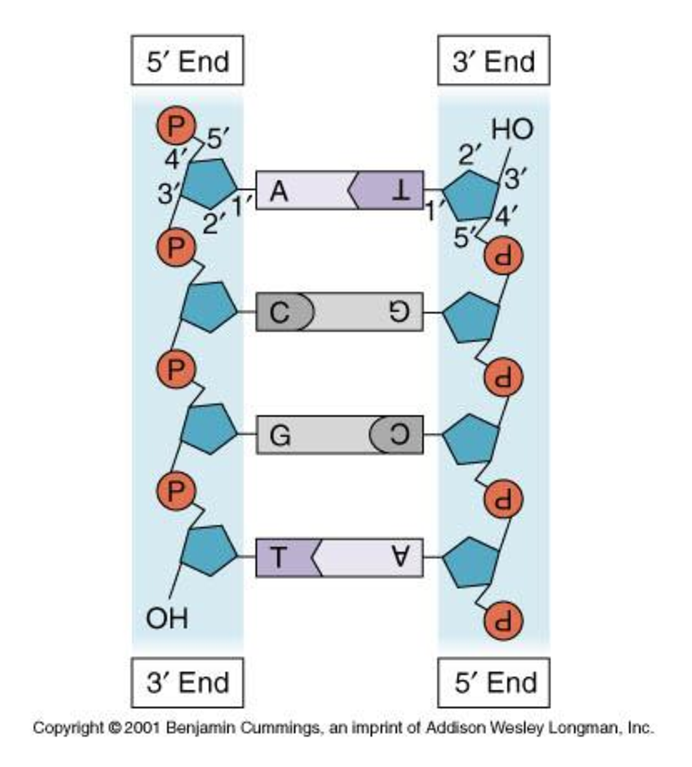
\includegraphics[width=0.4\textwidth]{graphics/dna_directionality.eps}
  \caption{DNA directionality}
  \label{fig:eukaryotic_cell}
\end{figure}
\FloatBarrier

\subsubsection{DNA replication}

\begin{itemize}
  \item Replication is essential for organisms to reproduce
  \item Without replication, cell division could not occur
  \item Replication must be high fidelity but have potential for error (to
        enable evolution)
\end{itemize}

\Para{C-value paradox}

The C-value is the size of an organisms genome (defined as the amount of DNA in
pico grams in a haploid cell).

C-values not reflective of complexity, i.e. no relation between C-value and
number of genes.

\subsubsection{Genome structure}

\Para{Prokaryotic}

\begin{itemize}
  \item Generally small ($<10 \mathrm{M}$ bases)
  \item Single, circular chromosome
  \item Can have plasmids \\
        Disposable genetic elements that often carry genes for antibiotic
        resistance or toxicity
  \item Information dense \\
        Little or no space between genes, genes often overlap
  \item Genes are present in single, uninterrupted units
  \item Multiple genes may be present in single, uninterrupted units
\end{itemize}

\Para{Eukaryotic}

\begin{itemize}
  \item Usually larger than prokaryotic genomes
  \item Multiple, linear chromosomes
  \item Tend to be more information sparse \\
        Large gaps between genes
  \item Genes interrupted by non-coding sequence
    \begin{description}
      \item[Exons] coding
      \item[Introns] non-coding
    \end{description}
\end{itemize}

\subsubsection{DNA packaging}

Nuclear DNA is packaged as chromatin, a structure of DNA, RNA and protein.

Purpose of chromatin:
\begin{itemize}
  \item Packages DNA into a more compact structure
  \item Reinforces macromolecule to allow mitosis
  \item Prevents DNA damage
  \item Regulates gene expression and DNA replication
\end{itemize}

\begin{figure}[h!]
  \centering
  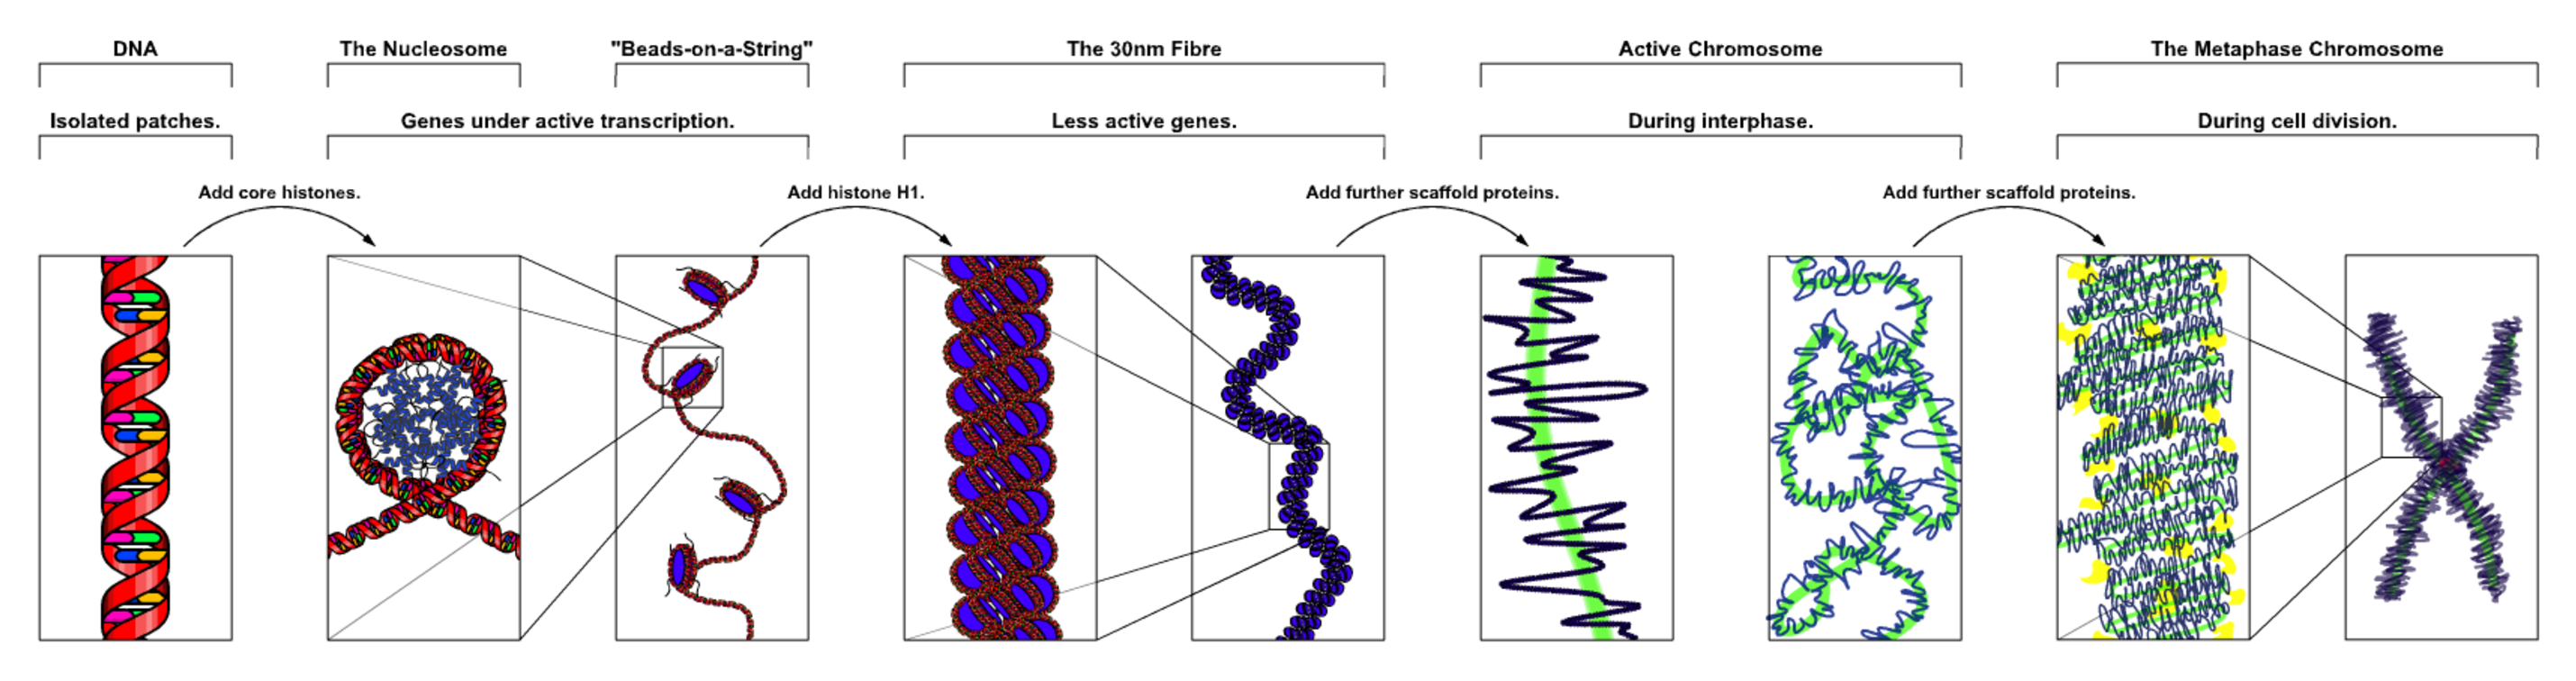
\includegraphics[width=\textwidth]{graphics/chromatin_structures.eps}
  \caption{Chromatin structure}
  \label{fig:chromatin_structures}
\end{figure}
\FloatBarrier

\subsubsection{Manipulating genomes}

\begin{itemize}
  \item Genetic engineering gives multiple techniques for editing the genome of
        an organism
  \item Simplest example is artificial selection to obtain desired traits
  \item Synthetic biology apples engineering principles to biology
\end{itemize}

\subsubsection{Gene structure}

\begin{itemize}
  \item Genes encode functional RNA modules
  \item A gene is a functional part of a chromosome
  \item Every cell contains the same set of genes
\end{itemize}

\subsection{Transcription}

Process of turning information stored in DNA into RNA.

\begin{description}
  \item[Non-template (coding) strand] \hfill \\
    Contains same base sequence as RNA crated
  \item[Template (non-coding) strand] \hfill \\
    Contains anti-codons of RNA
  \item[Promoter] \hfill \\
    Denotes start of RNA coding region
  \item[Coding region] \hfill \\
    RNA coding
  \item[Terminator] \hfill \\
    DNA coding denoting the end of the coding region
\end{description}

\begin{figure}[h!]
  \centering
  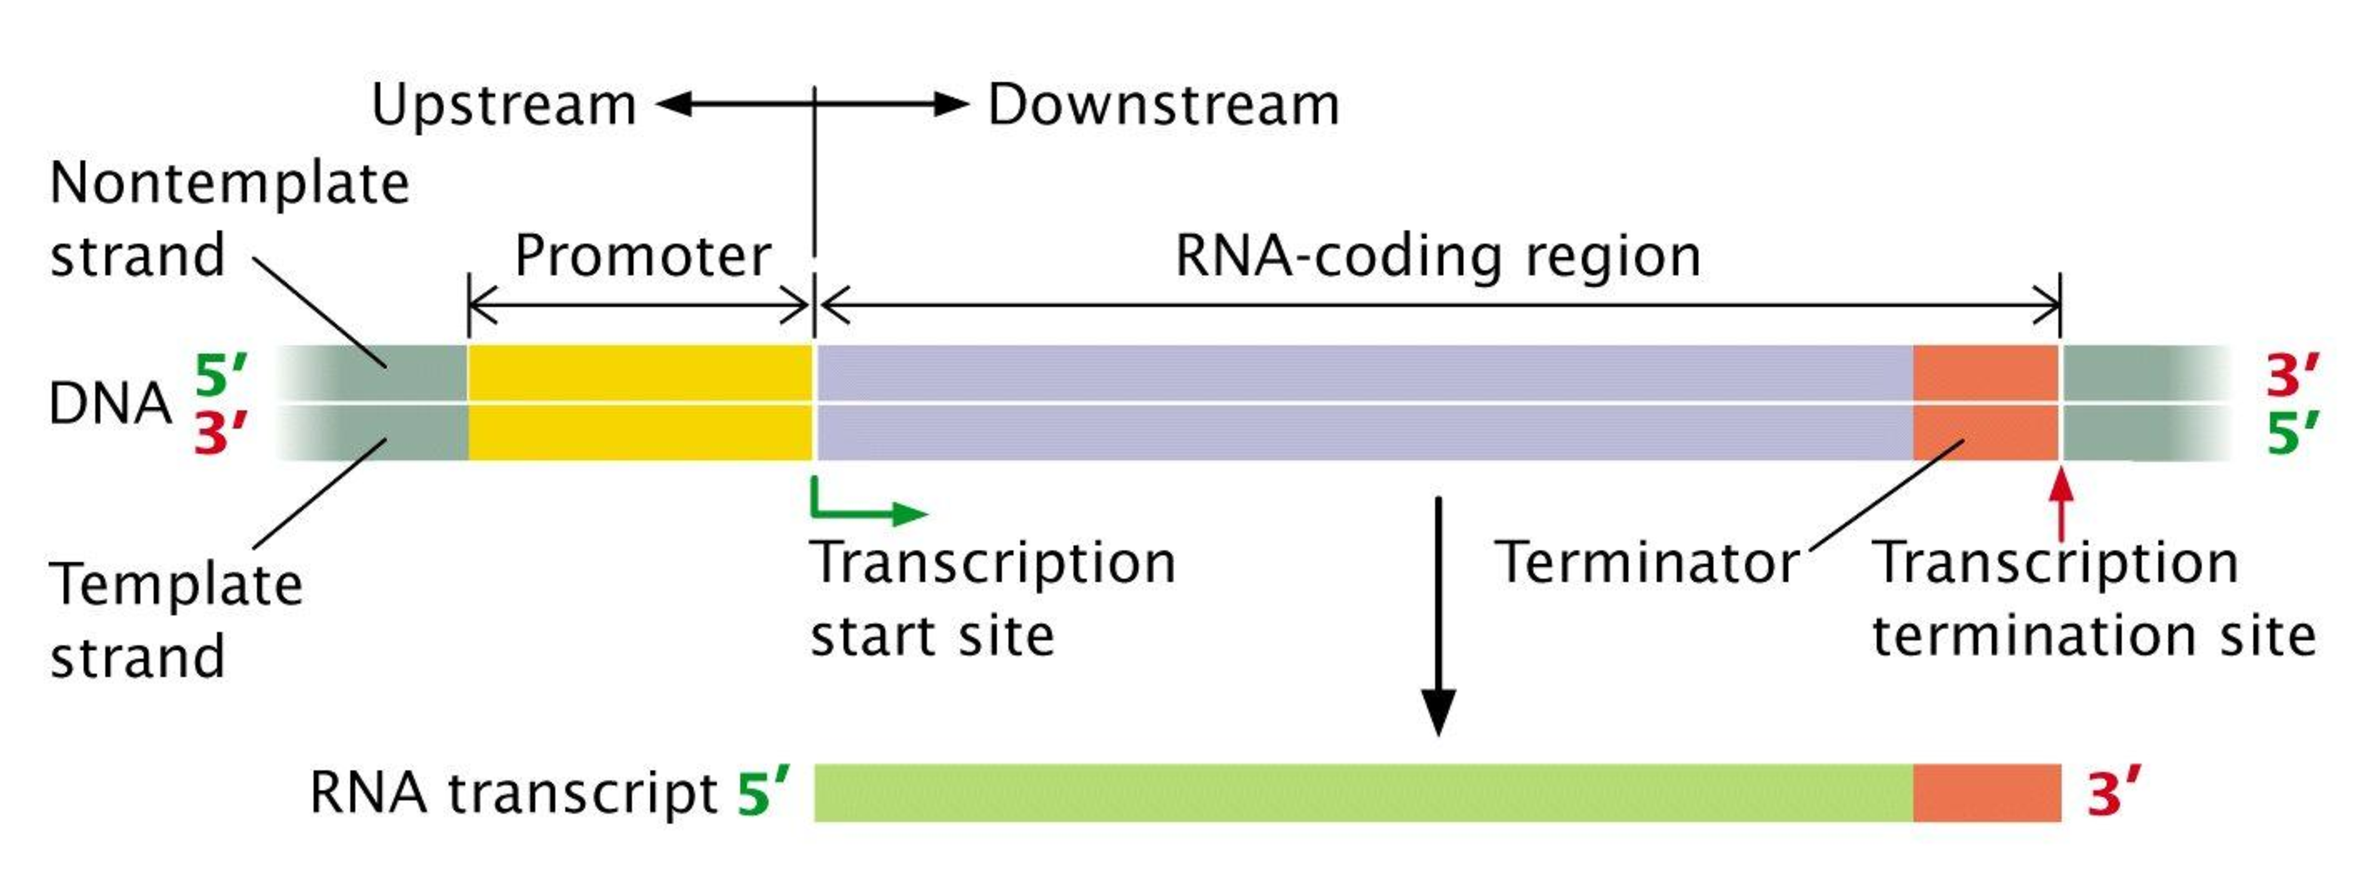
\includegraphics[width=0.8\textwidth]{graphics/dna-rna_transcription.eps}
  \caption{DNA directionality}
  \label{fig:dna-rna_transcription}
\end{figure}
\FloatBarrier

\begin{itemize}
  \item The base Thymine (T) in DNA is replaced with Uracil (U) in RNA
  \item Transcription occurs $5^{\prime}$ to $3^{\prime}$
  \item RNA polymerase is the enzyme responsible for transcription
  \item Transcription in eukaryotes is more complex
\end{itemize}

\subsubsection{Transcript processing}

Primary transcript must be processed into a mature message.

\begin{itemize}
  \item Addition of $5^{\prime}$ cap
    \begin{itemize}
      \item 7-methlyguanosine
      \item Involved in ribosome binding
      \item Protective
    \end{itemize}
  \item $3^{\prime}$ polyadenylation
    \begin{itemize}
      \item Addition of tail of adenosine to mRNA
      \item Required for nuclear export and stability
    \end{itemize}
  \item Splicing
    \begin{itemize}
      \item Primary transcript contains both introns and exons
      \item Introns must be removed
    \end{itemize}
\end{itemize}

\subsection{Translation}

The process of transforming the information contained in mRNA into an amino acid
chain, which is folded into a protein (amino acids joined by peptide bonds).

\begin{itemize}
  \item Proteins may be structural or have an active role (e.g. enzymes)
  \item Protein function sis determined by its amino acid sequence and its three
        dimensional structure
\end{itemize}

\subsubsection{RNA to protein}

Nucleotide sequence is read in groups of three (codon). Codons are consecutive
and non-overlapping.

Each codon corresponds to one of 20 amino acids.

Special cases:
\begin{description}
  \item[AUG]
    Methionine indicates start of frame
  \item[UAA]
    Frame terminator
  \item[UAG]
    Frame terminator
  \item[UGA]
    Frame terminator
\end{description}

\subsubsection{Amino acid structure}

\begin{itemize}
  \item Common structure to all amino acids
  \item Side chain defines properties of amino acid
\end{itemize}

\begin{figure}[h!]
  \centering
  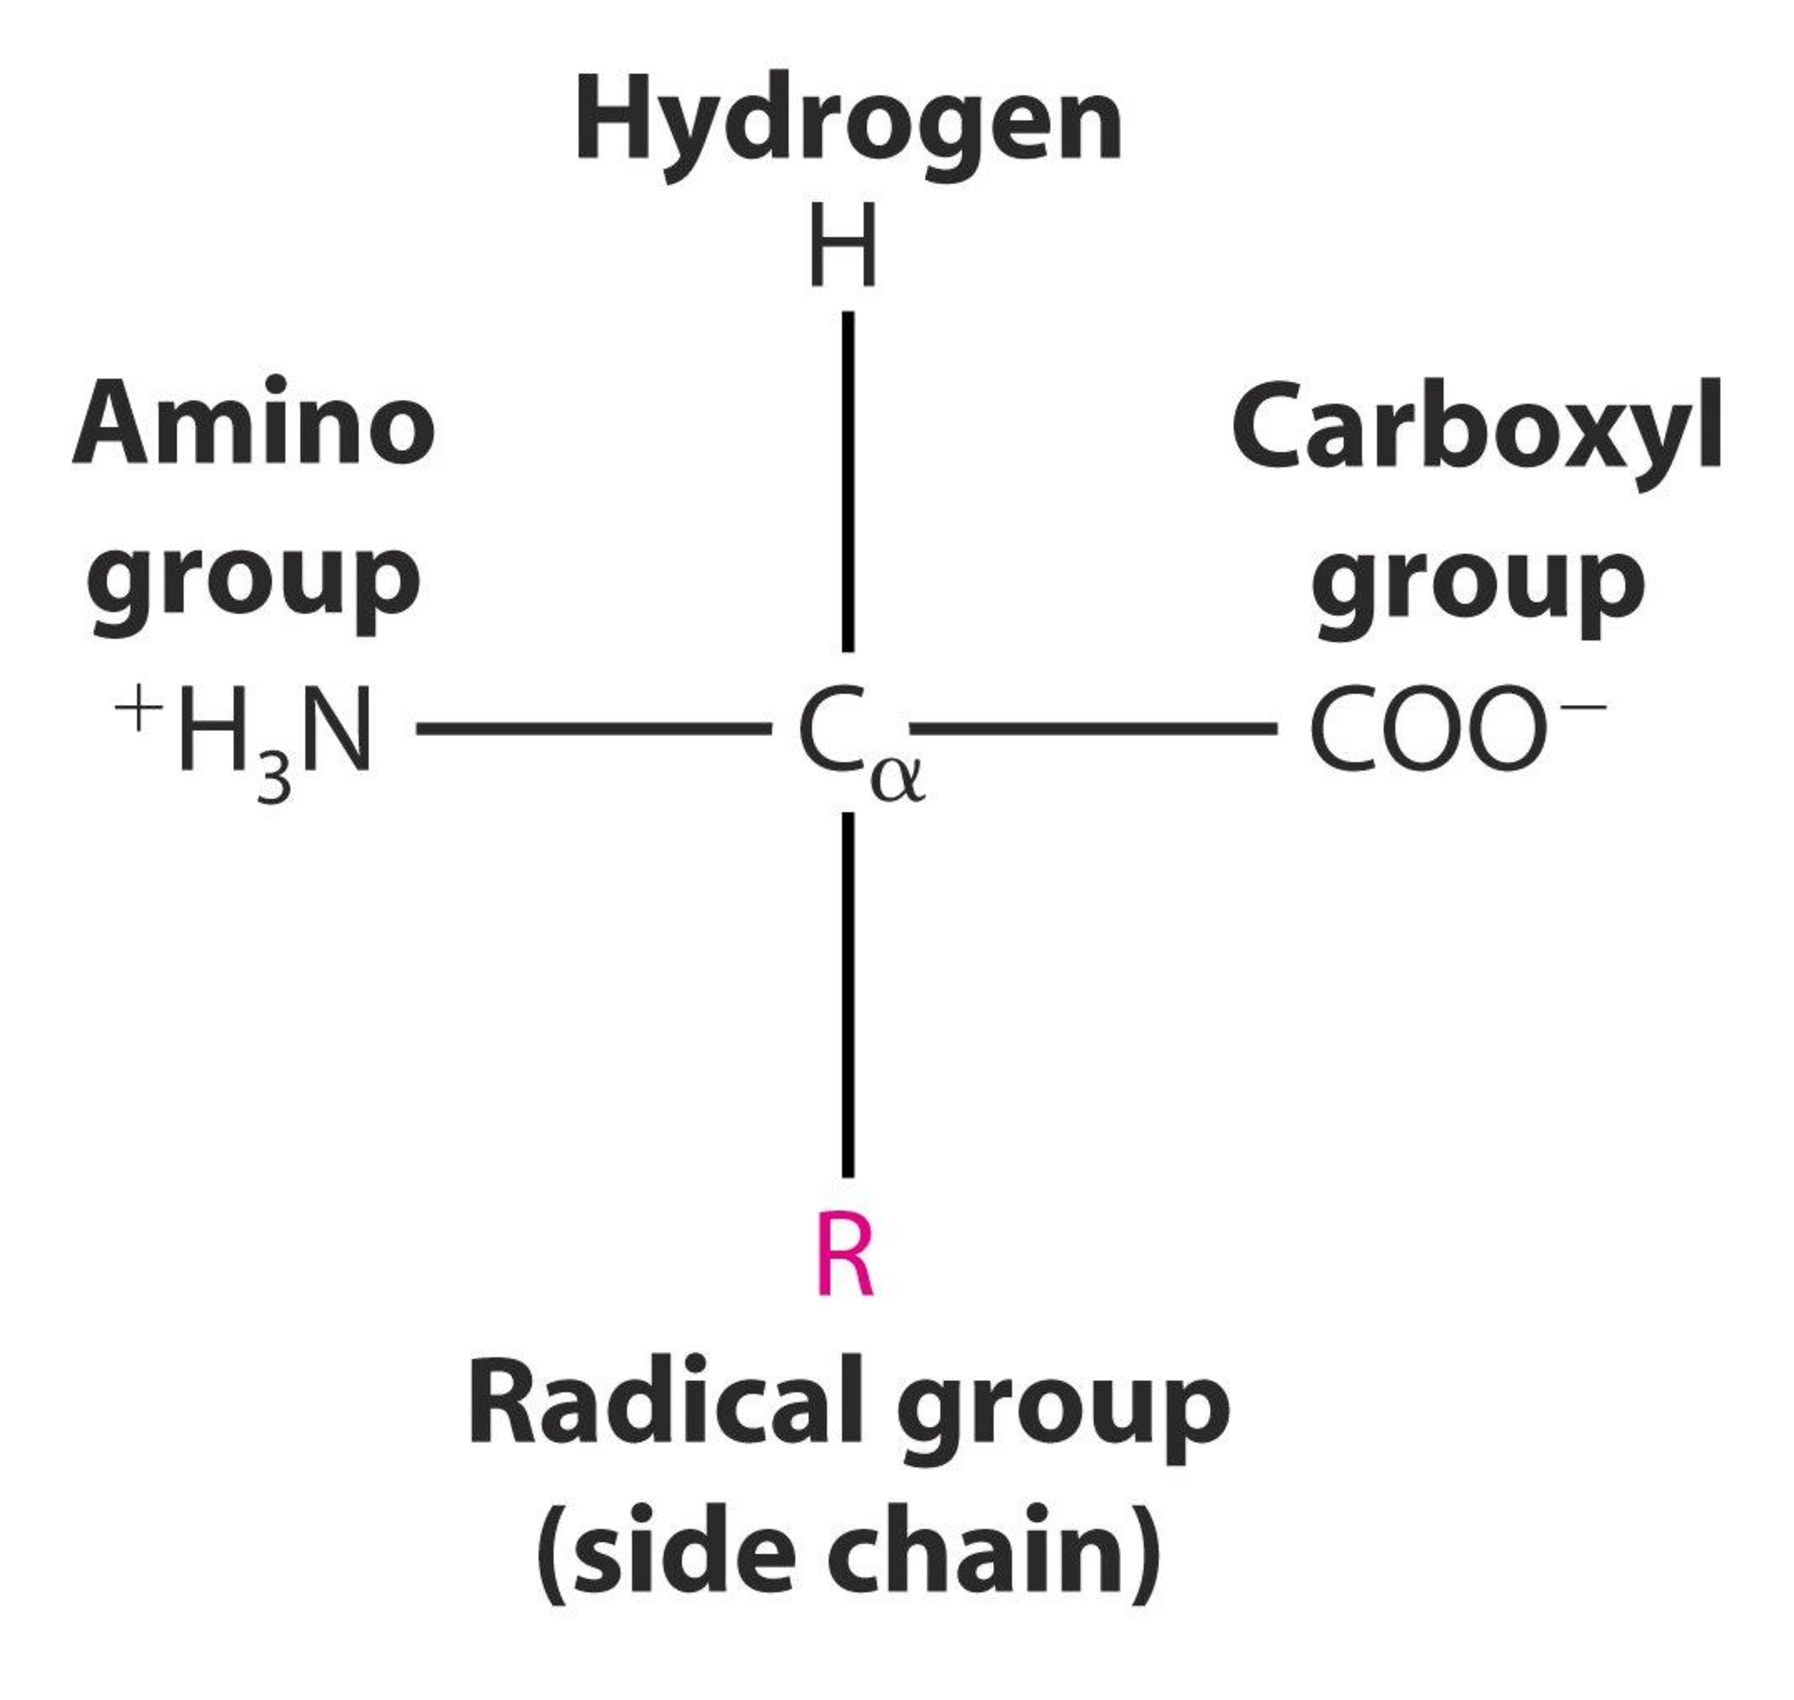
\includegraphics[width=0.35\textwidth]{graphics/amino_acid_structure.eps}
  \caption{Amino acid structure}
  \label{fig:amino_acid_structure}
\end{figure}
\FloatBarrier

Protein is constructed when multiple amino acids are combined into a string by a
peptide bond between the carboxyl group of one acid and the amino group of
another (giving $\mathrm{H}_{2}\mathrm{O}$ as a by-product).

\begin{figure}[h!]
  \centering
  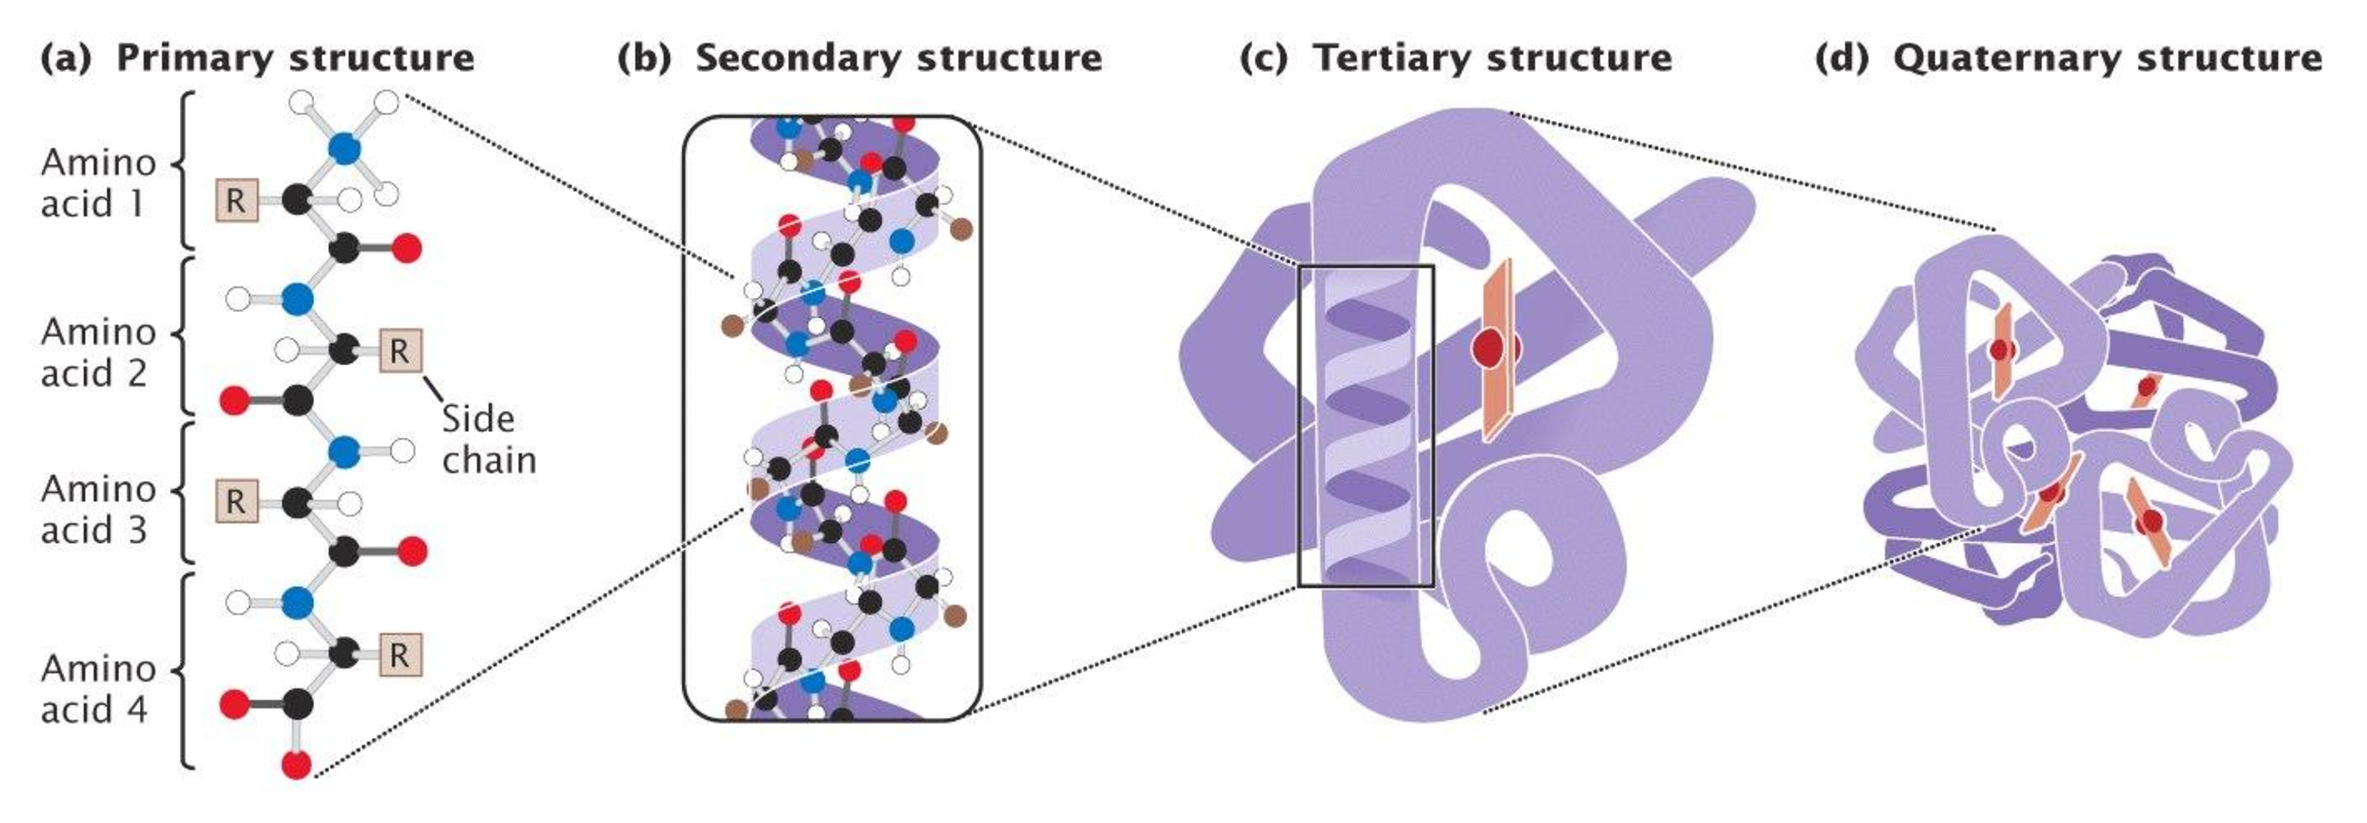
\includegraphics[width=\textwidth]{graphics/protein_structure.eps}
  \caption{Protein structure}
  \label{fig:protein_structure}
\end{figure}
\FloatBarrier

\subsubsection{Ribosomes}

\begin{itemize}
  \item Bind to the region of the mRNA that lies just upstream of the AUG codon
  \item Ribosome Binding Site (RBS) given a consensus sequence which varies with
        organism
\end{itemize}

\subsubsection{Translation process}

\begin{enumerate}
  \item[0] Binding of amino acid to tRNA
  \item[1] Initiation
    \begin{itemize}
      \item Ribosome recognition
        \begin{itemize}
          \item Prokaryotes: mRNA RBS hydrogen bonds with rRNA
          \item Eukaryotes: ribosome attaches to $5^{\prime}$ cap
        \end{itemize}
      \item $\mathrm{tRNA}^{\mathrm{met}}$ binds to AUG codon
    \end{itemize}
  \item[2] Elongation
  \item[3] Termination
    \begin{itemize}
      \item Ribosome pauses at stop codon
      \item Release factor binds
    \end{itemize}
\end{enumerate}

\subsubsection{Control of Gene Expression}

\begin{itemize}
  \item Various levels of control:
    \begin{itemize}
      \item Transcription
      \item Post-transcription
      \item Translation
      \item Post-translation
    \end{itemize}
\end{itemize}

\section{Genome Sequencing and Assembly}

\subsection{Sequencing}

Reasons for sequencing:

\begin{itemize}
  \item Identify content and structure
  \item Identify mutations
\end{itemize}

\subsubsection{Sanger sequencing}

\begin{itemize}
  \item
    Uses DNA polymerase to synthesise DNA

    Enzyme that when given a DNA strand will synthesise the complementary strand

  \item
    A mixture of the polymerase, a primer (small strand of complimentary DNA)
    and deoxynucleotides (DNA nucleotides with fluorescent tag) is made.

  \item
    Products then separated. Multiple methods exist but traditionally using gel
    electrophoresis which allows florescent markers to be seen in four distinct
    "lanes" corresponding to each DNA nucleotide.

  \item
    Accurate but slow

\end{itemize}

\subsubsection{454 pyro-sequencing}

\begin{itemize}
  \item High throughput and lower sample preparation time
\end{itemize}

\subsubsection{Illumina Solexa approach}

\begin{itemize}
  \item Sequencing based on synthesis
  \item Lower cost per sequenced base but high initial cost
\end{itemize}

\subsubsection{Nanopore}

\begin{itemize}
  \item
    Feed DNA through a pore in a surface and detect nucleotides as they pass
    through

  \item
    Faster with minimal sample preparation

\end{itemize}

\subsection{Assembly}

Sequencing produces several fragments of the full genome, in order to obtain the
sequence of the full genome such subsequences must be assembled.

\subsubsection{Shotgun sequencing}

\begin{itemize}
  \item
\end{itemize}

\subsubsection{Greedy assembly}

\begin{itemize}
  \item
\end{itemize}

\subsubsection{deBruijn assembly}

\begin{itemize}
  \item
\end{itemize}

\subsection{Tools and Resources}

\subsubsection{Databases}

\begin{description}
  \item[European Neucleotide Archive (ENA)] \hfill \\
    European Bioinformatics Institute database \\
    \url{http://www.ebi.ac.uk/ena}
  \item[GenBank] \hfill \\
    National Center for Biotechnology Information (NCBI) (US) database \\
    \url{http://www.ncbi.nlm.nih.gov/genbank/}
  \item[DBA Data Bank of Japan (DDBJ)] \hfill \\
    National Institute of Genetics (NIG) (Japan) database \\
    \url{http://www.ddbj.nig.ac.jp/}
\end{description}

\subsubsection{Browsers}

\begin{description}
  \item[Ensembl Genome Browser] \hfill \\
    \url{http://www.ensembl.org/index.html}
  \item[UCSC Genome Browser] \hfill \\
    \url{https://genome.ucsc.edu/}
\end{description}

\section{Evolution and its effects}

TODO

\section{Transcriptions and Proteomes}

TODO

\end{document}
